\section{Auswertung}
\label{sec:Auswertung}
\subsection{Durchbiegung des runden Stabes}
Der runde Stab weißt folgende Daten und Abmessungen auf
\begin{align*}
    \text{Länge: } l&=\qty{0,589(0.001)}{\meter},\\
    \text{Durchmesser: } d&=\qty{1,0(0,1)e-3}{\meter}\text{ und}\\
    \text{Masse: } m&=\qty{0,4116(0.0001)}{\kilo\gram}.
\end{align*}
Daraus ergibt sich für das Volumen und die Dichte 
\begin{align*}
    V&=\qty{4.6(0.05)e-5}{\meter\cubed}\text{ und}\\
    \rho&=\qty{8.9(0.09)e3}{\kilo\gram\per\meter\cubed}.
\end{align*}
Die Fehler werden über Pythons Applikation \textit{SciPy} via der Gaußschen 
Fehlerforpflanzung berechnet
\begin{equation}
    \increment f=\sqrt{\sum_{k=1}^{n}\biggl(\frac{\partial f}{\partial x_\text{k}}\biggr)^2(\increment x_\text{k})^2}\,.
    \label{eq:gauss}
    \end{equation}
Dabei ist $f$ die zur Berechnung der Größe gegebene Formel und $x_k$ dessen Argumente.
$\increment x_k$ ist der jeweilige Fehler der einzelnen Argumente.\\ 
Mittelwerte, Standardabweichungen und sonstige Fehler werden für diesen Versuch alle mit Python bzw. 
numeric python berechnet. \noindent 
Der Wert der Dichte entspricht dem Literaturwert von $\qty{8,92}{\kilo\gram\per\meter\cubed}$ für Kupfer \cite{Kupfer}. 
Auch das äußere Erscheinungsbild deutet auf Kupfer hin.
\subsubsection{Einseitige Einspannung}
Für die einseitige Einspannung des Stabes ergeben sich die in \autoref{tab:rund1} 
aufgeführten Messwerte. Der Stab ist bei $L=\qty{51,5}{\centi\meter}$ eingespannt.
\begin{table}
    \centering
    \caption{Abstand zur Einspannung, Auslenkung mit und ohne Gewicht sowie deren Differenz.}
    \label{tab:rund1}
    \begin{tblr}{colspec={c c c c||c c c c}}
        \toprule
        $x$\ /\ cm & $D_0$\ /\ mm & $D_\text{Gewicht}$\ /\ mm & $\increment D$&
        $x$\ /\ cm & $D_0$\ /\ mm & $D_\text{Gewicht}$\ /\ mm & $\increment D$\\
        \midrule
        50 & 5.71 & 2.47 & 3.24 & 26 & 7.10 & 5.91 & 1.19\\
        47 & 5.90 & 3.06 & 2.84 & 23 & 7.24 & 6.28 & 0.96\\
        44 & 6.29 & 4.40 & 1.89 & 20 & 7.35 & 6.58 & 0.77\\
        41 & 6.38 & 3.92 & 2.46 & 17 & 7.47 & 6.89 & 0.58\\
        38 & 6.53 & 4.32 & 2.21 & 14 & 7.57 & 7.17 & 0.40\\
        35 & 6.76 & 4.81 & 1.95 & 11 & 7.69 & 7.41 & 0.28\\
        32 & 6.90 & 5.17 & 1.73 & 08  & 7.78 & 7.61 & 0.17\\
        29 & 7.00 & 5.55 & 1.45 & 05  & 7.82 & 7.74 & 0.08\\
        \bottomrule
    \end{tblr}
\end{table}
Es sollen nun die Elastizitätsmodule der Stäbe bestimmt werden. Dafür wird jeweils eine lineare Regression der Form
$l(x)=ax+b$ durch die Messwerte gelegt, welche nach Gleichung \eqref{eq:polynom1} lineariesiert werden. Der Vorfaktor 
$\sfrac{F}{2EI}$ des Polynoms $Lx^2-\sfrac{x^3}{3}$ ist dabei die Steigung der Ausgleichsgeraden. Dieses Verfahren und 
die Bennenung der jeweiligen Koeffizienten bleibt für jede Teilberechnung dieses Protokolls gleich. Da $F$ und $I$ 
aus den gegebenen Größen direkt berechnet werden können, kann $a=\sfrac{F}{2EI}$ direkt nach dem Elastizitätsmodul $E$
umgestellt werden. Das Flächenträgheitsmoment $I$ wird über $I_\circ=\sfrac{\pi d^4}{64}$ berechnet \cite{Flächenträgheitsmomente}. In 
\autoref{fig:plota} sind die Messwerte der ersten Messreihe sowie die lineare Regression zu sehen. Die angehangene 
Masse beträgt $m=\qty{0,5}{\kilo\gram}$\,.
\begin{figure}[H]
    \centering
    \caption{Messwerte des einseitig eingespannten runden Stabes und deren lineare Regression.}
    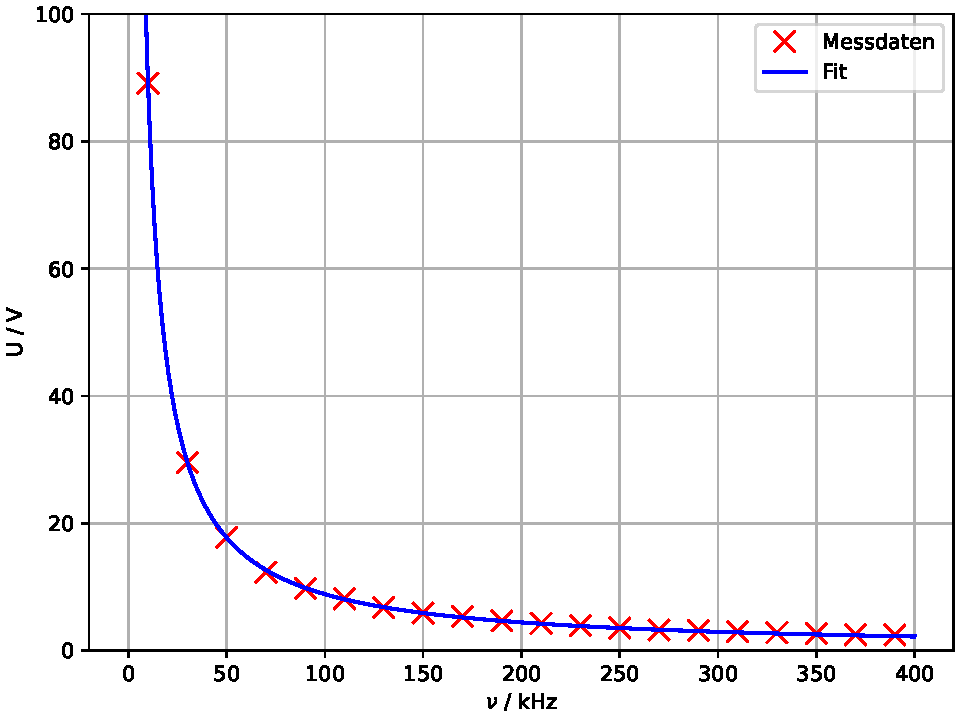
\includegraphics[width=\textwidth]{build/plota.pdf}
    \label{fig:plota}
\end{figure}
Für die Koeffizienten ergeben sich mit \textit{Python} die Werte
\begin{align*}
    a&=\qty{3,4(0,19)e-2}{\per\meter\squared}\text{ und}\\
    b&=\qty{1,4(0,9)e-4}{\meter}.
\end{align*}
Der Elastizitätsmodul berechnet sich über
\begin{align*}
E&=\frac{F}{2aI}
\intertext{mit}
F&=mg=\qty{0,5}{\kilo\gram}\cdot\qty{9,806}{\meter\per\second\squared} \text{ und } I=\qty{4,91e-10}{\meter\tothe{4}}
\intertext{zu}
E_{\circ,\text{einseitig}}&=\qty{146(8,2)}{\giga\pascal}\,.
\end{align*}
\subsubsection{Beideitig Einspannung}
Zur beidseitigen Einspannung des runden Stabes ergeben sich die in \autoref{tab:rund2} aufgeführten Messwerte.
\begin{table}
    \centering
    \caption{Messwerte der Durchbiegung eines runden Stabes links und rechts der Mitte mit und ohne Gewicht.}
    \label{tab:rund2}
    \begin{tblr}{colspec={c c c c c c c c}}
        \toprule
        $x_\text{l}$\ /\ cm & $x_\text{r}$\ /\ cm  & $D_{0\text{l}}$\ /\ mm & $D_\text{Gewicht,l}$\ /\ mm &
        $D_{0\text{r}}$\ /\ mm & $D_\text{Gewicht,r}$\ /\ mm & $\increment D_\text{l}$ & $\increment D_\text{r}$ \\
        \midrule
        31 & 24 & 7.16 & 7.61 & 6.89 & 7.36 & 0.27 & 0.25\\
        32 & 23 & 7.17 & 7.60 & 6.93 & 7.39 & 0.24 & 0.20\\
        33 & 22 & 7.18 & 7.63 & 6.83 & 7.40 & 0.35 & 0.23\\
        34 & 21 & 7.15 & 7.65 & 6.89 & 7.44 & 0.26 & 0.21\\
        35 & 20 & 7.14 & 7.64 & 6.88 & 7.44 & 0.26 & 0.20\\
        37 & 18 & 7.14 & 7.65 & 6.89 & 7.46 & 0.25 & 0.19\\
        39 & 16 & 7.13 & 7.72 & 6.90 & 7.68 & 0.23 & 0.04\\
        41 & 14 & 7.11 & 7.75 & 6.89 & 7.61 & 0.22 & 0.14\\
        43 & 12 & 7.08 & 7.77 & 6.89 & 7.69 & 0.19 & 0.08\\
        45 & 10 & 7.02 & 7.82 & 6.86 & 7.74 & 0.16 & 0.08\\
        47 & 08 & 7.06 & 7.83 & 6.93 & 7.77 & 0.13 & 0.06\\
        \bottomrule
    \end{tblr}
\end{table}
Aus diesen Messwerten lassen sich zwei Plots erstellen und damit zwei mal der Elastizitätsmodul bestimmen.
\autoref{fig:plotb} zeigt die lineare Regression sowie die Messdaten der rechten Seite, \autoref{fig:plotc} 
die der linken. Für die Messwerte der rechten Seite ($x\leq\sfrac{L}{2}$) wird die $x$-Skala nach Formel 
\eqref{eq:rechts} skaliert, für die linke Seite nach Formel \eqref{eq:links}.
Das Gewicht ist bei dieser Messreihe mittig bei $\qty{27,75}{\centi\meter}$ angebracht und hat eine Masse
von $\qty{1}{\kilo\gram}$\,. 
\begin{figure}[H]
    \centering
    \caption{Messwerte sowie die lineare Regression der Durchbiegung des beidseitig eingespannten runden Stabes rechtsseitig.}
    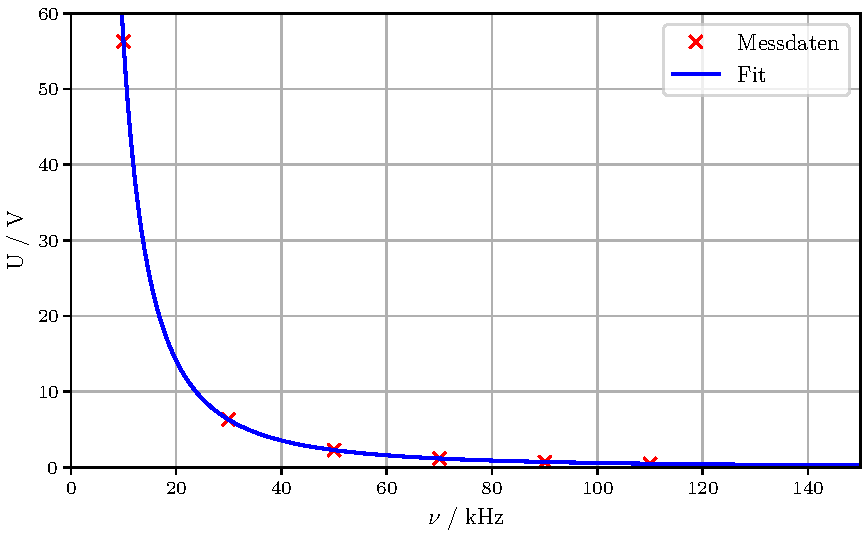
\includegraphics[width=\textwidth]{build/plotb.pdf}
    \label{fig:plotb}
\end{figure}
Für die rechte Seite ergeben sich die Koeffizienten 
\begin{align*}
    a&=\qty{2(0.4)e-3}{\per\meter\squared}\text{ und}\\
    b&=\qty{-1.1(0.6)e-4}{\meter}\,.
\end{align*}
Über das gleiche Vorgehen wie bei einseitiger Einspannung ergibt sich der Elastizitätsmodul. Der einzige Unterschied ist 
der Vorfaktor des Polynoms $D(x)$ nach Gleichung \eqref{eq:rechts} und \eqref{eq:links}. Der Wert für $E$ berechnet sich zu
\begin{equation*}
E_{\circ,\text{beidseitig,rechts}}=\qty{2.1(0.4)e2}{\giga\pascal}\,.
\end{equation*}
\begin{figure}[H]
    \centering
    \caption{Messwerte sowie die lineare Regression der Durchbiegung des beidseitig eingespannten runden Stabes linksseitig.}
    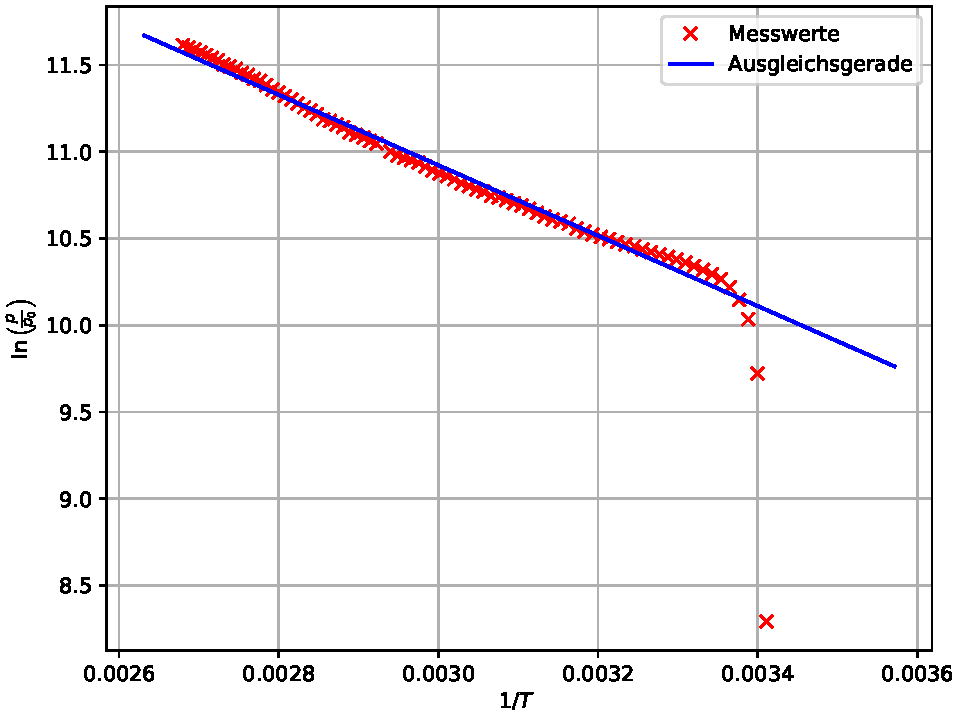
\includegraphics[width=\textwidth]{build/plotc.pdf}
    \label{fig:plotc}
\end{figure}
Für die linke Seite ergeben sich die Koeffizienten
\begin{align*}
    a&=\qty{1,6(0.29)e-3}{\per\meter\squared}\text{ und}\\
    b&=\qty{8(3)e-5}{\meter}\,.
\end{align*}
Damit ergibt sich der Elastizitätsmodul für die linke Seite
\begin{equation*}
    E_{\circ,\text{beidseitig,links}}=\qty{2.6(0.5)e2}{\giga\pascal}\,.
\end{equation*}
\subsection{Quadratischer Stab}
Für den qaudratischen Stab verläuft die Auswertung analog. Das Flächenträgheitsmoment für den quardatischen Stab errechnet sich
über $I_\square=\sfrac{d^4}{12}$. Der qaudratische Stab hat die Abmessungen 
\begin{align*}
    \text{Länge: } l&=\qty{0,6(0.001)}{\meter},\\
    \text{Dicke: } d&=\qty{1,0(0,1)e-3}{\meter}\text{ und}\\
    \text{Masse: } m&=\qty{0,5357(0.0001)}{\kilo\gram}.
\end{align*}
Daraus ergibt sich für das Volumen und die Dichte 
\begin{align*}
    V&=\qty{6(0.06)e-5}{\meter\cubed}\text{ und}\\
    \rho&=\qty{8.93(0.09)e3}{\kilo\gram\per\meter\cubed}.
\end{align*}
Auch dieser Stab ist aus Kupfer gefertigt, da wieder das äußere Erscheinungsbild sowie die Dichte darauf schließen lässt \cite{Kupfer}.
\subsubsection{Einseitige Einspannung}
Für die einseitige Einspannung des Stabes ergeben sich die in \autoref{tab:quadr1} 
aufgeführten Messwerte. Auch dieser Stab ist bei $L=\qty{51,5}{\centi\meter}$ eingespannt.
\begin{table}
    \centering
    \caption{Abstand zur Einspannung, Auslenkung mit und ohne Gewicht sowie deren Differenz des quadratischen Stabes.}
    \label{tab:quadr1}
    \begin{tblr}{colspec={c c c c||c c c c}}
        \toprule
        $x$\ /\ cm & $D_0$\ /\ mm & $D_\text{Gewicht}$\ /\ mm & $\increment D$&
        $x$\ /\ cm & $D_0$\ /\ mm & $D_\text{Gewicht}$\ /\ mm & $\increment D$\\
        \midrule
        49 & 4.74 & 2.51 & 2.23 & 25 & 6.47 & 5.74 & 0.73\\
        46 & 4.93 & 3.03 & 1.90 & 22 & 6.65 & 6.05 & 0.60\\
        43 & 5.21 & 3.43 & 1.78 & 19 & 6.77 & 6.31 & 0.46\\
        40 & 5.43 & 3.82 & 1.61 & 16 & 6.95 & 6.63 & 0.32\\
        37 & 5.66 & 4.24 & 1.42 & 13 & 7.12 & 6.87 & 0.25\\
        34 & 5.89 & 4.65 & 1.24 & 10 & 7.27 & 7.12 & 0.15\\
        31 & 6.10 & 5.06 & 1.04 & 07 & 7.40 & 7.32 & 0.08\\
        28 & 6.32 & 5.43 & 0.89 & 04 & 7.50 & 7.46 & 0.04\\
        \bottomrule
    \end{tblr}
\end{table}
Erneut wird der Elastizitätsmodul nach gleicher Berechnungsvorschrift wie für den runden Stab ermittelt. In \autoref{fig:plotd}
ist die zu den Koeffizienten 
\begin{align*}
    a&=\qty{2.6(0.03)e-2}{\per\meter\squared}\,\,\text{und}\\
    b&=\qty{4(1)e-5}{\meter}
\end{align*}
gehörende lineare Regression sowie die in der Tabelle \ref{tab:quadr1} aufgeführten Messdaten zu sehen.
\begin{figure}[H]
    \centering
    \caption{Messwerte des einseitig eingespannten quadratischen Stabes und deren lineare Regression.}
    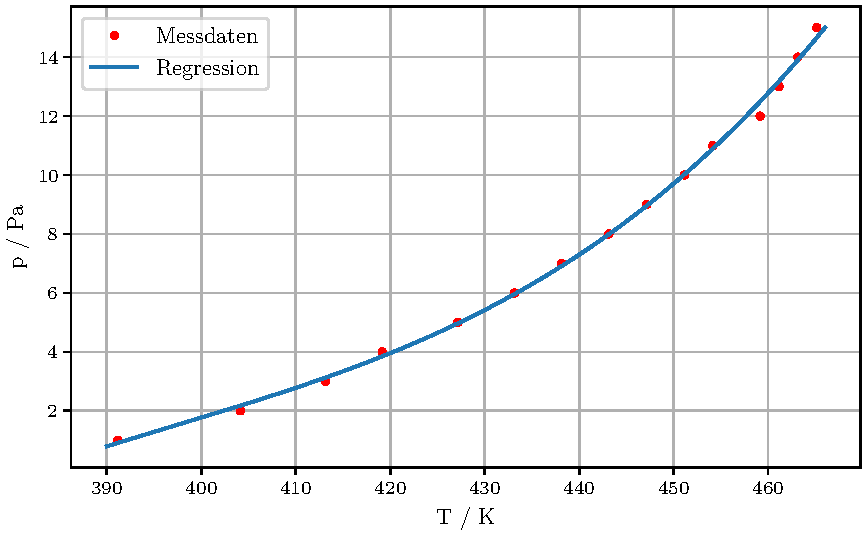
\includegraphics[width=\textwidth]{build/plotd.pdf}
    \label{fig:plotd}
\end{figure}
Der Elastizitätsmodul errechnet sich zu 
\begin{equation*}
    E_{\square,\text{einseitig}}=\qty{1,13(0.026)e2}{\giga\pascal}\,.
\end{equation*}
\subsubsection{Beidseitige Einspannung}
Für die beidseitige Einspannung des qaudratischen Stabes ergeben sich die in Tabelle \ref{tab:quadr2} aufgeführten Messwerte.
Das Gewicht wurde wieder mit einer Masse von $m=\qty{1}{\kilo\gram}$ mittig aufgehangen.
\begin{table}
    \centering
    \caption{Messwerte der Durchbiegung eines quadratischen Stabes links und rechts der Mitte mit und ohne Gewicht.}
    \label{tab:quadr2}
    \begin{tblr}{colspec={c c c c c c c c}}
        \toprule
        $x_\text{l}$\ /\ cm & $x_\text{r}$\ /\ cm  & $D_{0\text{l}}$\ /\ mm & $D_\text{Gewicht,l}$\ /\ mm &
        $D_{0\text{r}}$\ /\ mm & $D_\text{Gewicht,r}$\ /\ mm & $\increment D_\text{l}$ & $\increment D_\text{r}$ \\
        \midrule
        31 & 24 & 7.91 & 8.00 & 7.83 & 7.93 & 0.08 & 0.07\\
        33 & 22 & 7.97 & 7.94 & 7.98 & 7.86 & -0.01 & 0.08\\
        35 & 20 & 8.18 & 7.88 & 8.08 & 7.79 & 0.10 & 0.09\\
        37 & 18 & 8.26 & 7.79 & 8.18 & 7.73 & 0.08 & 0.04\\
        39 & 16 & 8.35 & 7.81 & 8.27 & 7.75 & 0.08 & 0.06\\
        41 & 14 & 8.43 & 7.77 & 8.36 & 7.73 & 0.07 & 0.04\\
        43 & 12 & 8.54 & 7.76 & 8.48 & 7.72 & 0.06 & 0.04\\
        45 & 10 & 8.55 & 7.76 & 8.53 & 7.72 & 0.02 & 0.04\\
        47 & 08 & 8.73 & 7.74 & 8.69 & 7.72 & 0.04 & 0.04\\
        49 & 06 & 8.75 & 7.71 & 8.72 & 7.70 & 0.03 & 0.01\\
        \bottomrule
    \end{tblr}
\end{table}
Die Koeffizienten zur linearen Reggression in Abbildung \ref{fig:plote} sind
\begin{align*}
    a&=\qty{5.3(1.2)e-4}{\per\meter\squared} \text{ und }\\
    b&=\qty{1(1)e-5}{\meter}\,.
\end{align*}
\begin{figure}[H]
    \centering
    \caption{Messwerte des beidseitig eingespannten quadratischen Stabes und deren lineare Regression rechtsseitig.}
    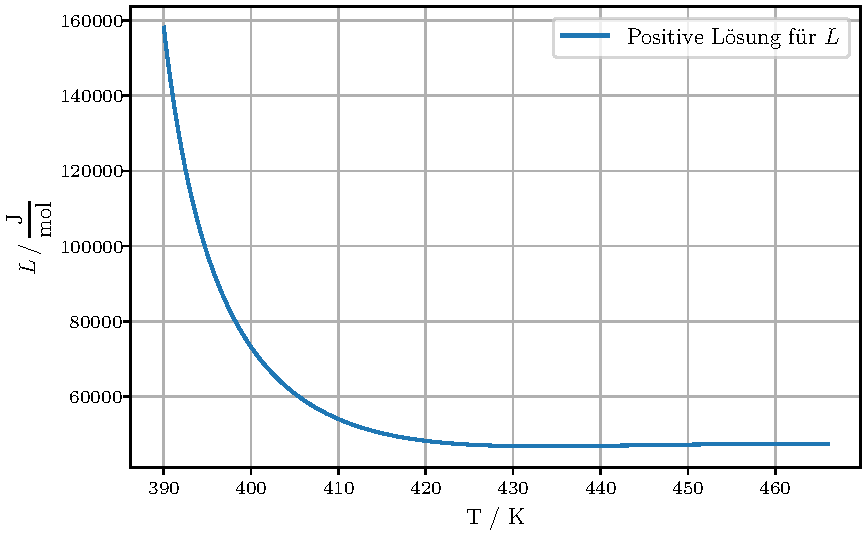
\includegraphics[width=\textwidth]{build/plote.pdf}
    \label{fig:plote}
\end{figure}
Dazu ergibt sich der Elastizitätsmodul 
\begin{equation*}
    E_{\square,\text{beidseitig, rechts}}=\qty{4.6(1.1)e2}{\giga\pascal}\,.
\end{equation*}
Schließlich sind die Koeffizienten zur linearen Reggression in Abbildung \ref{fig:plotf} 
\begin{align*}
    a&=\qty{6.2(0.6)e-4}{\per\meter\squared} \text{ und }\\
    b&=\qty{2(1)e-5}{\meter}\,.
\end{align*}
\begin{figure}[H]
    \centering
    \caption{Messwerte des beidseitig eingespannten quadratischen Stabes und deren lineare Regression linksseitig.}
    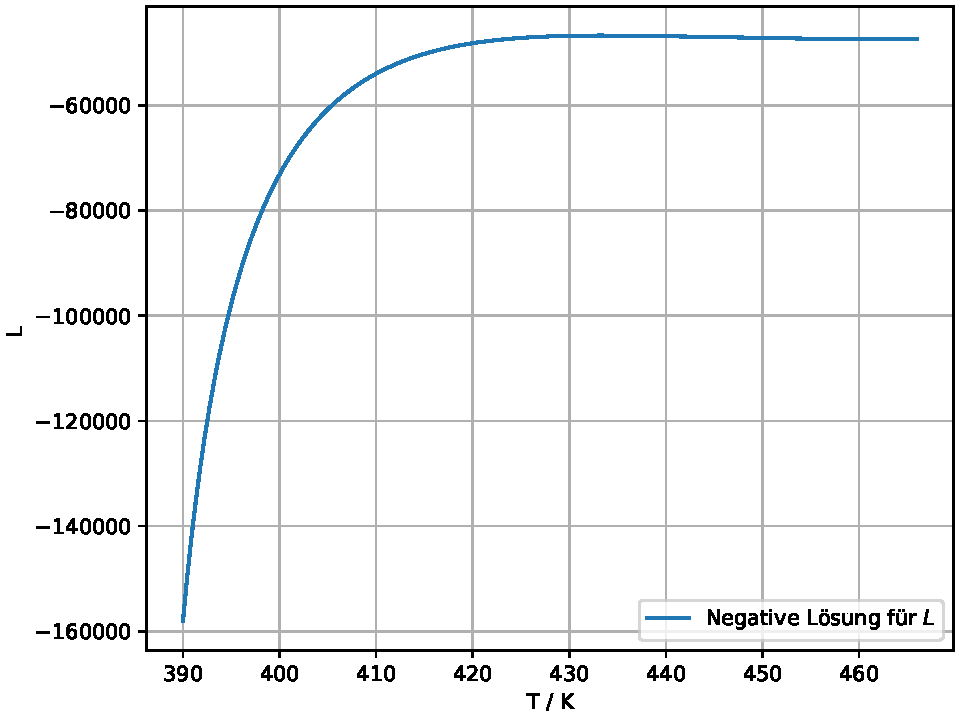
\includegraphics[width=\textwidth]{build/plotf.pdf}
    \label{fig:plotf}
\end{figure}
Dazu ergibt sich der letzte Elastizitätsmodul 
\begin{equation*}
    E_{\square,\text{beidseitig, links}}=\qty{4(4)e2}{\giga\pascal}\,.
\end{equation*}